% Adjust these for the path of the theme and its graphics, relative to this file
%\usepackage{beamerthemeFalmouthGamesAcademy}
\usepackage{../../beamerthemeFalmouthGamesAcademy}
\usepackage{multimedia}
\graphicspath{ {../../} }

% Default language for code listings
\lstset{language=C++,
        morekeywords={each,in,nullptr}
}

% For strikethrough effect
\usepackage[normalem]{ulem}
\usepackage{wasysym}

\usepackage{pdfpages}

% http://www.texample.net/tikz/examples/state-machine/
\usetikzlibrary{arrows,automata}

\newcommand{\modulecode}{COMP260}\newcommand{\moduletitle}{Distributed Systems}\newcommand{\sessionnumber}{5}

\begin{document}
\title{\sessionnumber: Session title here}
\subtitle{\modulecode: \moduletitle}

\frame{\titlepage} 

\begin{frame}
	\frametitle{Learning outcomes}
	\begin{itemize}
		\item Outcome 1
		\item Outcome 2
		\item Outcome 3
	\end{itemize}
\end{frame}

\begin{frame}
	\frametitle{acuity}
	
\end{frame}

\begin{frame}
	\frametitle{Cones and Rods}
	\begin{figure}
		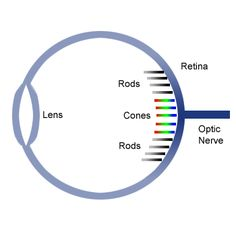
\includegraphics[scale=.5]{assets/cones-rods.jpg}
		\caption{ Fovea }
	\end{figure}
\end{frame}

\begin{frame}
	\frametitle{Foveated Rendering}
	\begin{center}
		\href{https://www.youtube.com/watch?v=6q3w0fiD0zg}{ 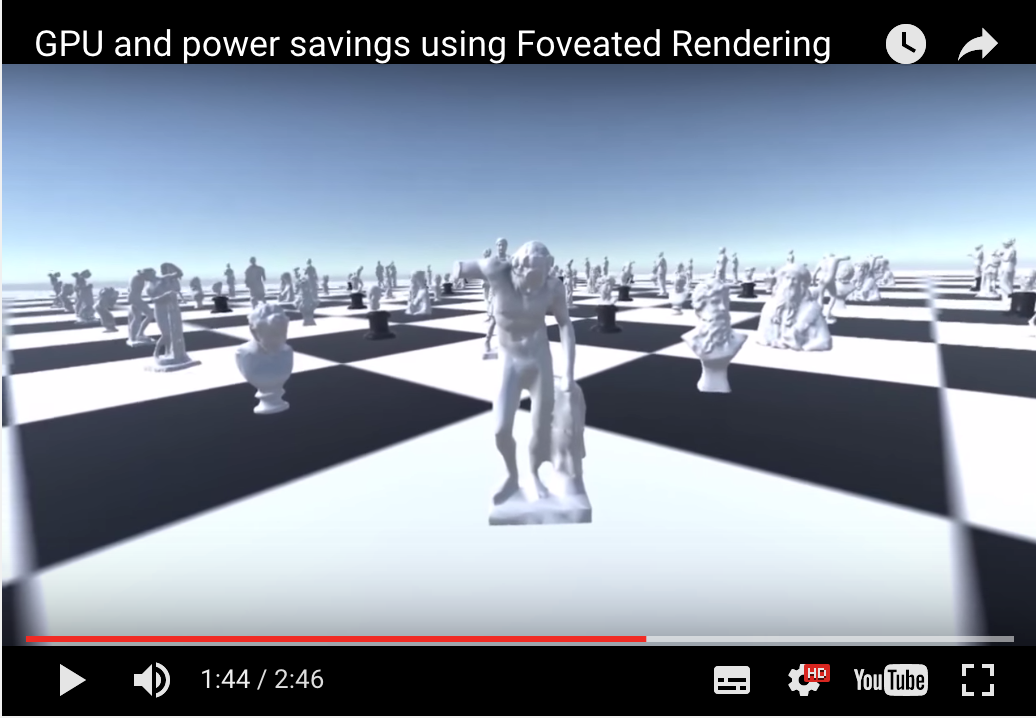
\includegraphics[scale=.4]{assets/foveated-rendering}  }
	\end{center}
\end{frame}

\end{document}
